%!TEX root = ../operads_paper.tex
\section{Action operads}
This chapter will give an introduction to the basic theory of operads (cite MAY), before introducing the notion of an action operad (\ref{Defi:aop}) and exploring some of the consequences of this definition. QQQ WRITE MORE
\subsection{Introduction to operads}
This section will provide an introduction to operads, including a general overview of the definitions of plain, symmetric, and braided operads. Remarks and examples are provided throughout and the section begins with conventions around notation.

We begin with the basic definitions. The diagrams for the axioms in some operadic definitions can look quite involved and we recommend that readers expand the products depicted, or write out a small example case, to better see what the axioms are describing.

\begin{Defi}
A \textit{symmetric operad} $O$ (in the category of sets) consists of
\begin{itemize}
\item a set, $O(n)$, for each natural number $n$,
\item for each $n$, a right $\Sigma_{n}$-action on $O(n)$,
\item an element $\id \in O(1)$, and
\item functions
  \[
    \mu \colon  O(n) \times O(k_{1}) \times \cdots \times O(k_{n}) \rightarrow O(k_{1} + \cdots + k_{n}),
  \]
\end{itemize}
satisfying the following three axioms.
\begin{enumerate}
\item The element $\id \in O(1)$ is a two-sided unit for $\mu$ in the sense that
  \begin{align*}
    \mu(\id;x) &= x\\
    \mu(x;\id,\ldots,\id) &= x
  \end{align*}
for any $x \in O(n)$.
\item The functions $\mu$ (called operadic multiplication or operadic composition) are associative in the sense that the diagram below commutes.
% \[
% \xy
% (0,0)*+{\scriptstyle O(n) \times O(k_{1}) \times \cdots \times O(k_{n}) \times O(l_{1,1}) \times \cdots \times O(l_{{1},k_{1}}) \times \cdots \times O(l_{n,1}) \times \cdots \times O(l_{{n},k_{n}})} ="00";
% (0,-50)*+{\scriptstyle O(k_{1} + \cdots + k_{n}) \times O(l_{1,1}) \times \cdots \times O(l_{{1},k_{1}}) \times \cdots \times O(l_{n,1})\times \cdots \times O(l_{{n},k_{n}})} ="02";
% (55,-10)*+{\scriptstyle O(n) \times \prod_{i=1}^n O(k_{i}) \times O(l_{i,1}) \times \cdots \times O(l_{{i}, k_{i}}) } ="20";
% (55,-25)*+{\scriptstyle O(n) \times O(\sum l_{1,-}) \times \cdots \times O(\sum l_{n,-})} ="21";
% (55, -40)*+{\scriptstyle  O(\sum l_{-,-})} ="22";
% {\ar_{\scriptstyle \mu \times 1} "00" ; "02"};
% {\ar_{\mu} "02" ; "22"};
% {\ar^{\cong} "00" ; "20"};
% {\ar^{1 \times \prod \mu} "20" ; "21"};
% {\ar^{\mu} "21" ; "22"};
% \endxy
% \]


  \[
    \xy
      (0,0)*+{\scriptstyle O(n) \times \left(\prod_{i=1}^n O(k_i)\right) \times \left(\prod_{i=1}^n\prod_{j=1}^{k_i} O(l_{i,j})\right)}="a";
      (65,0)*+{\scriptstyle O(n) \times \prod_{i=1}^n \left(O(k_i) \times \prod_{j=1}^{k_i} O(l_{i,j})\right)}="b";
      (65,-20)*+{\scriptstyle O(n) \times \prod_{i=1}^n O\left(\sum_{j=1}^{k_i} l_{i,j}\right)}="c";
      (65,-40)*+{\scriptstyle O\left(\sum_{i=1}^n \sum_{j=1}^{k_i} l_{i,j}\right)}="d";
      (0,-40)*+{\scriptstyle O\left(\sum_{i=1}^n k_i\right) \times \prod_{i=1}^n \prod_{j=1}^{k_i} O(l_{i,j})}="e";
      %
      {\ar^{\cong} "a" ; "b"};
      {\ar^{1 \times \prod \mu} "b" ; "c"};
      {\ar^{\mu} "c" ; "d"};
      {\ar_{\mu \times 1} "a" ; "e"};
      {\ar_{\mu} "e" ; "d"};
    \endxy
  \]

\item The functions $\mu$ are equivariant with respect to the symmetric group actions, and so satisfies the following two equations.
  \begin{align*}
    \mu(x;y_1 \cdot \tau_1,\ldots,y_n \cdot \tau_n) &= \mu(x;y_1,\ldots,y_n)\cdot \beta(\tau_1,\ldots,\tau_n)\\
    \mu(x \cdot \sigma; y_1, \ldots, y_n) &= \mu\left(x;y_{\sigma^{-1}(1)},\ldots,y_{\sigma_{-1}(n)}\right)\cdot \delta(\sigma)
  \end{align*}
  % \begin{align*}
  %   \mu(x;y_1 \cdot \tau_1,\ldots,y_n \cdot \tau_n) &= \mu(x;y_1,\ldots,y_n)\cdot(\tau_1 \oplus \ldots \oplus \tau_n)\\
  %   \mu(x \cdot \sigma; y_1, \ldots, y_n) &= \mu\left(x;y_{\sigma^{-1}(1)},\ldots,y_{\sigma_{-1}(n)}\right)\cdot \sigma^+
  % \end{align*}
\end{enumerate}
\end{Defi}

\begin{rem}
It is useful to write out in full what the sets in the diagram of the second axiom above mean. The use of numerous products and indices is to save space but the full picture becomes much clearer when these are expanded. For the equations in the third axiom above to make sense, we must have
\begin{itemize}
\item $x \in O(n)$,
\item $y_{i} \in O(k_{i})$ for $i=1, \ldots, n$,
\item $\tau_{i} \in \Sigma_{k_{i}}$,
\item $\sigma \in \Sigma_{n}$, and
\item $\beta(\tau_1,\ldots,\tau_n), \delta(\sigma) \in \Sigma_{k_1 + \ldots + k_n}$ as described in \cref{conv1} and in \cref{exSigma} below.
\end{itemize}

\end{rem}
\begin{Defi}
A \emph{non-symmetric operad} $O$ consists of the same data as above but without any symmetric group actions, and only satisfying the first and second axioms.
\end{Defi}

\begin{rem}
\begin{enumerate}
\item One can change from operads in $\mb{Sets}$ to operads in another symmetric monoidal category $\mathcal{V}$ by requiring each $O(n)$ to be an object of $\mathcal{V}$ and replacing all instances of cartesian product with the appropriate tensor product in $\mathcal{V}$. This includes replacing the element $\id \in O(1)$ with a map $I \rightarrow O(1)$ from the unit object of $\mathcal{V}$ to $O(1)$.
\item Every symmetric operad has an underlying \textit{symmetric collection} which consists of the natural number-indexed set $\{ O(n) \}_{n \in \N}$ together with symmetric group actions, but without a chosen identity element or composition maps. The category of symmetric collections is a presheaf category, and we will equip it with a monoidal structure in which monoids are precisely operads in \cref{operad=monoid}. A similar construction, but without reference to group actions, shows that every non-symmetric operad has an underlying (non-symmetric) collection which is now merely a $\N$-indexed collection of sets.
\end{enumerate}
\end{rem}

One is intended to think that $x \in O(n)$ is a function with $n$ inputs and a single output, as below.
  \begin{center}
  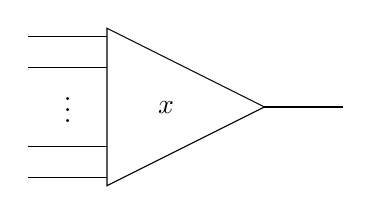
\begin{tikzpicture}
    \draw (0,0.9) -- (1,0.9);
    \draw (0,0.5) -- (1,0.5);
    %
    \node [anchor=center] () at (0.5,0) {$\vdots$\strut};
    %
    \draw (0,-0.5) -- (1,-0.5);
    \draw (0,-0.9) -- (1,-0.9);
    %
    \draw (1,1) -- (1,-1) -- (3,0) -- cycle;
    %
    \draw (3,0) -- (4,0);
    %
    \node [anchor=center] () at (1.75,0) {$x$\strut};
  \end{tikzpicture}
  \end{center}
  % \[
  %   \xy
  %     {\ar@{-} (0,0)*{}; (25,-10)*{} };
  %     {\ar@{-} (0,-20)*{}; (25,-10)*{} };
  %     {\ar@{-} (0,0)*{}; (0,-20)*{} };
  %     {\ar@{-} (25,-10)*{}; (35,-10)*{} };
  %     {\ar@{-} (0,0)*{}; (-10,0)*{} };
  %     {\ar@{-} (0,-3)*{}; (-10,-3)*{} };
  %     {\ar@{-} (0,-17)*{}; (-10,-17)*{} };
  %     {\ar@{-} (0,-20)*{}; (-10,-20)*{} };
  %     (11,-10)*{x}; (-5,-10)*{\vdots}
  %   \endxy
  % \]
Operadic composition is then a generalization of function composition, with the pictorial representation below being $\mu(x; y_{1}, y_{2})$ for $\mu \colon O(2) \times O(2) \times O(3) \rightarrow O(5)$.
  \begin{center}
  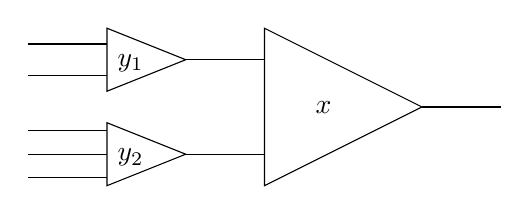
\begin{tikzpicture}
    % upper triangle
    \draw (-2,0.8) -- (-1,0.8);
    %
    \draw (-2,0.4) -- (-1,0.4);
    %
    \draw (-1,1) -- (-1,0.2) -- (0,0.6) -- cycle;
    %
    \node [anchor=center] () at (-0.7,0.6) {$y_1$\strut};    
    % lower triangle
    \draw (-2,-0.9) -- (-1,-0.9);
    %
    \draw (-2,-0.3) -- (-1,-0.3);
    %
    \draw (-1,-1) -- (-1,-0.2) -- (0,-0.6) -- cycle;
    %
    \draw (-2,-0.6) -- (-1,-0.6);
    %
    \node [anchor=center] () at (-0.7,-0.6) {$y_2$\strut};
    % big triangle
    \draw (0,0.6) -- (1,0.6);
    %    
    \draw (0,-0.6) -- (1,-0.6);
    %
    \draw (1,1) -- (1,-1) -- (3,0) -- cycle;
    %
    \draw (3,0) -- (4,0);
    %
    \node [anchor=center] () at (1.75,0) {$x$\strut};
  \end{tikzpicture}
  \end{center}
  % \[
  %   \xy
  %     {\ar@{-} (0,0)*{}; (25,-10)*{} };
  %     {\ar@{-} (0,-20)*{}; (25,-10)*{} };
  %     {\ar@{-} (0,0)*{}; (0,-20)*{} };
  %     {\ar@{-} (25,-10)*{}; (35,-10)*{} };
  %     {\ar@{-} (0,-3)*{}; (-10,-3)*{} };
  %     {\ar@{-} (0,-17)*{}; (-10,-17)*{} };
  %     (11,-10)*{x};
  %     {\ar@{-} (-25,2)*{}; (-10,-3)*{} };
  %     {\ar@{-} (-25,-8)*{}; (-10,-3)*{} };
  %     {\ar@{-} (-25,2)*{}; (-25,-8)*{} };
  %     {\ar@{-} (-25,1)*{}; (-30,1)*{} };
  %     {\ar@{-} (-30,-7)*{}; (-25,-7)*{} };
  %     (-19,-3)*{y_{1}};
  %     {\ar@{-} (-25,-12)*{}; (-10,-17)*{} };
  %     {\ar@{-} (-25,-22)*{}; (-10,-17)*{} };
  %     {\ar@{-} (-25,-12)*{}; (-25,-22)*{} };
  %     {\ar@{-} (-25,-13)*{}; (-30,-13)*{} };
  %     {\ar@{-} (-25,-17)*{}; (-30,-17)*{} };
  %     {\ar@{-} (-25,-21)*{}; (-30,-21)*{} };
  %     (-19,-17)*{y_{2}};
  %   \endxy
  % \]

\begin{example}\label{exSigma}
The canonical example of an operad is the symmetric operad which we write as $\Sigma$. The set $\Sigma(n)$ is the set of elements of the symmetric group $\Sigma_{n}$, and the group action is just multiplication on the right. The identity element $\id \in \Sigma(1)$ is just the identity permutation on a one-element set. Operadic composition in $\Sigma$ will then be given by a function
  \[
    \Sigma(n) \times \Sigma(k_{1}) \times \cdots \times \Sigma(k_{n}) \rightarrow \Sigma(k_{1} + \cdots + k_{n})
  \]
which takes permutations $\sigma \in \Sigma_{n}, \tau_{i} \in \Sigma_{k_{i}}$ and produces the following permutation in $\Sigma_{k_{1} + \cdots + k_{n}}$. First we form the block sum permutation $\beta(\tau_1,\ldots,\tau_n)$ which permutes the first $k_{1}$ elements according to $\tau_{1}$, the next $k_{2}$ elements according to $\tau_{2}$ and so on; this is an element of $\Sigma_{k_{1} + \cdots + k_{n}}$. Then we take the permutation $\delta(\sigma) \in \Sigma_{k_{1} + \cdots + k_{n}}$ which permutes the $n$ different blocks $1$ through $k_{1}$, $k_{1}+1$ through $k_{1} + k_{2}$, and so on, according to the permutation $\sigma \in \Sigma_{n}$. Operadic composition in $\Sigma$ is then given by the formula
  \[
    \mu(\sigma; \tau_{1}, \ldots, \tau_{n}) = \delta(\sigma) \cdot \beta(\tau_1,\ldots,\tau_n).
  \]
Below we have drawn the permutation for the composition
  \[
    \mu \colon \Sigma(3) \times \Sigma(2) \times \Sigma(4) \times \Sigma(3) \rightarrow \Sigma(9)
  \]
evaluated on the element $\left( (123); (12), (12)(34), (13) \right)$.
  \begin{center}
  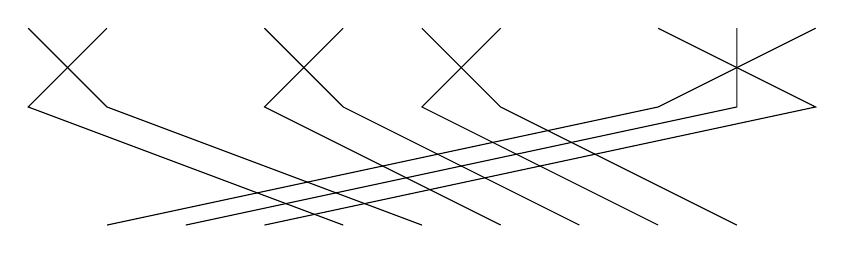
\begin{tikzpicture}
  \draw (1,0) -- (2,-1) -- (6,-2.5);
  \draw (2,0) -- (1,-1) -- (5,-2.5);
  \draw (4,0) -- (5,-1) -- (8,-2.5);
  \draw (5,0) -- (4,-1) -- (7,-2.5);
  \draw (6,0) -- (7,-1) -- (10,-2.5);
  \draw (7,0) -- (6,-1) -- (9,-2.5);
  \draw (9,0) -- (11,-1) -- (4,-2.5);
  \draw (10,0) -- (10,-1) -- (3,-2.5);
  \draw (11,0) -- (9,-1) -- (2,-2.5);
  \end{tikzpicture}
  \end{center}
  % \[
  %   \xy
  %     {\ar@{-} (0,0)*{}; (5,-5)*{} };
  %     {\ar@{-} (5,0)*{}; (0,-5)*{} };
  %     {\ar@{-} (12,0)*{}; (17,-5)*{} };
  %     {\ar@{-} (17,0)*{}; (12,-5)*{} };
  %     {\ar@{-} (22,0)*{}; (27,-5)*{} };
  %     {\ar@{-} (27,0)*{}; (22,-5)*{} };
  %     {\ar@{-} (34,0)*{}; (44,-5)*{} };
  %     {\ar@{-} (39,0)*{}; (39,-5)*{} };
  %     {\ar@{-} (44,0)*{}; (34,-5)*{} };
  %     {\ar@{-} (0,-5)*{}; (17,-13)*{} };
  %     {\ar@{-} (5,-5)*{}; (22,-13)*{} };
  %     {\ar@{-} (12,-5)*{}; (29,-13)*{} };
  %     {\ar@{-} (17,-5)*{}; (34,-13)*{} };
  %     {\ar@{-} (22,-5)*{}; (39,-13)*{} };
  %     {\ar@{-} (27,-5)*{}; (44,-13)*{} };
  %     {\ar@{-} (34,-5)*{}; (0,-13)*{} };
  %     {\ar@{-} (39,-5)*{}; (5,-13)*{} };
  %     {\ar@{-} (44,-5)*{}; (10,-13)*{} };
  %   \endxy
  % \]
Note that $(12)(34) \in \Sigma(4)$ is actually $\mu(e_{2}; (12), (12))$, where $e_{2} \in \Sigma_{2}$ is the identity permutation. Using this and operad associativity, one can easily check that
  \[
    \mu \left( (123); (12), (12)(34), (13) \right) = \mu \left( (1234); (12), (12), (12), (13) \right),
  \]
where now the composition on the right side uses the function
  \[
    \mu \colon \Sigma(4) \times \Sigma(2) \times \Sigma(2) \times \Sigma(2) \times \Sigma(3) \rightarrow \Sigma(9).
  \]
This equality is obvious using the picture above, but verifiable directly using only the algebra of the symmetric operad.
\end{example}


In the original topological applications \cite{maygeom}, symmetric operads were the central figures. A further kind of operad was studied by Fiedorowicz in \cite{fie-br}; we give the definition below in analogy with that for symmetric operads, with interpretation to follow afterwards to make it entirely rigorous. We do this to emphasize the key features that we will generalize in \cref{Defi:aop}.

\begin{Defi}\label{broperad}
A \textit{braided operad} consists of
  \begin{itemize}
    \item a non-symmetric operad $O$ and
    \item for each $n$, a right action of the $n$th braid group $B_{n}$ on $O(n)$,
  \end{itemize}
satisfying the following axioms.
  \begin{align*}
    \mu(x;y_1 \cdot \tau_1,\ldots,y_n \cdot \tau_n) &= \mu(x;y_1,\ldots,y_n)\cdot\beta(\tau_1,\ldots,\tau_n)\\
    \mu(x \cdot \sigma; y_1, \ldots, y_n) &= \mu\left(x;y_{\sigma^{-1}(1)},\ldots,y_{\sigma^{-1}(n)}\right)\cdot \delta(\sigma)
  \end{align*}
For the above equations to make sense, we must have
  \begin{itemize}
      \item $x \in O(n)$,
      \item $y_{i} \in O(k_{i})$ for $i=1, \ldots, n$,
      \item $\tau_{i} \in B_{k_{i}}$, and
      \item $\sigma \in B_{n}$.
  \end{itemize}
\end{Defi}

In order to make sense of this definition, we must define $\beta(\tau_1,\ldots,\tau_n)$ and $\delta(\sigma)$ in the context of braids. The first is the block sum in the obvious sense:  given $n$ different braids on $k_{1}, \ldots, k_{n}$ strands, respectively, we form a new braid on $k_{1} + \cdots + k_{n}$ strands by taking a disjoint union where the braid $\tau_{i}$ is to the left of $\tau_{j}$ if $i < j$. The braid $\delta(\sigma)$ is obtained by replacing the $i$th strand with $k_{i}$ consecutive strands, all of which are braided together according to $\sigma$.

We require one final preparatory definition.

\begin{Defi}\label{Defi:op_map}
Let $O,O'$ be operads. Then an \textit{operad map} $f \colon O \rightarrow O'$ consists of functions $f_{n} \colon O(n) \rightarrow O'(n)$ for each natural number such that the following axioms hold.

  \begin{align*}
    f\left(\id_O\right) &= \id_{O'}\\
    f\left(\mu^{O}(x;y_1,\ldots,y_n)\right) &= \mu^{O'}\left(f(x);f(y_1),\ldots,f(y_n)\right)
  \end{align*}
The maps $f_{n}$ are required to be equivariant with respect to the symmetric group actions if $f$ is to be a map of symmetric operads, or braid actions if $f$ is to be a map of braided operads.
\end{Defi}

\begin{conv}
In the above definition and below, we adopt the convention that if an equation requires using operadic composition in more than one operad, we will indicate this by a superscript on each instance of $\mu$ unless it is entirely clear from context.
\end{conv}

\begin{example}
One can form an operad $B$ where $B(n)$ is the underlying set of the $n$th braid group, $B_{n}$. This is done in much the same way as we did for the symmetric operad, and the collection of maps $\pi_{n} \colon B_{n} \rightarrow \Sigma_{n}$ giving the underlying permutations constitutes an operad map (of non-symmetric or braided operads) operads $Br \rightarrow \Sigma$.
\end{example}

\subsection{Action operads}

 	% QQQ chapter: action operads
 	% \begin{itemize}
 	% 	\item defines action operads 
 	% 	\item considers familiar examples including symmetric, braided and ribbon braided
 	% 	\item remarks about terminal and initial action operads
 	% 	\item introduction of action operad maps
  %   \item Possibly cite Yau around here (or in the introduction?)
 	% \end{itemize}

One should note that the axioms for symmetric and braided operads each use the fact that the groups of equivariance themselves form an operad. This is what we call an action operad and we remark on similar structures defined and studied by others. After introducing the basic definition, we will consider familiar examples, such as those just noted, as well as less familiar examples such as those constituted by ribbon braid groups or so-called `cactus' groups. We then proceed with some remarks about terminal and initial action operads, as well as maps between action operads.

\begin{Defi}\label{Defi:aop}
An \textit{action operad} $\Lambda$ consists of
\begin{itemize}
\item an operad $\Lambda = \{ \Lambda(n) \}$ in the category of sets such that each $\Lambda(n)$ is equipped with the structure of a group and
\item a map $\pi \colon \Lambda \rightarrow \Sigma$ which is simultaneously a map of operads and a group homomorphism $\pi_{n} \colon \Lambda(n) \rightarrow \Sigma_{n}$ for each $n$
\end{itemize}
such that one additional axiom holds. Write
  \[
    \mu \colon  \Lambda(n) \times \Lambda(k_{1}) \times \cdots \times \Lambda(k_{n}) \rightarrow \Lambda(k_{1} + \cdots + k_{n})
  \]
for the multiplication in the operad $\Lambda$. Let $(g; f_1, \ldots, f_n)$ be an element of the product $\Lambda(n) \times \Lambda(k_{1}) \times \cdots \times \Lambda(k_{n})$ and let $(g'; f_1', \ldots f_n')$ be an element of the product $\Lambda(n) \times \Lambda(k_{g^{-1}(1)}) \times \cdots \times \Lambda(k_{g^{-1}(1)})$. We require that
  \begin{eqn}\label{eqn:ao_axiom}
    \mu\left(g'; f_1', \ldots f_n'\right)  \mu\left(g; f_1, \ldots, f_n\right) = \mu\left(g'g; f_{g(1)}'f_{1}, \ldots, f_{g(n)}'f_{n}\right)
  \end{eqn}
in the group $\Lambda(k_{1} + \cdots + k_{n})$.
\end{Defi}

\begin{rem}
\begin{itemize}
\item As per  \cref{conv1}, we write $g(i)$ to mean $\pi(g)(i)$ and $g^{-1}(i)$ to mean $\pi(g)^{-1}(i)$, where this is obvious from context.  
\item The final axiom is best explained using the operad $\Sigma$ of symmetric groups. Reading symmetric group elements as permutations from top to bottom, below is a pictorial representation of the final axiom for the map $\mu \colon \Sigma_{3} \times \Sigma_{2} \times \Sigma_{2} \times \Sigma_{2} \rightarrow \Sigma_{6}.$
  % \[
  %   \xy
  %     {\ar@{-} (0,0)*{}; (5,-5)*{} };
  %     {\ar@{-} (5,-5)*{}; (29,-10)*{} };
  %     {\ar@{-} (5,0)*{}; (0,-5)*{} };
  %     {\ar@{-} (0,-5)*{}; (24,-10)*{} };
  %     {\ar@{-} (12,0)*{}; (12,-5)*{} };
  %     {\ar@{-} (12,-5)*{}; (0,-10)*{} };
  %     {\ar@{-} (17,0)*{}; (17,-5)*{} };
  %     {\ar@{-} (17,-5)*{}; (5,-10)*{} };
  %     {\ar@{-} (24,0)*{}; (29,-5)*{} };
  %     {\ar@{-} (29,-5)*{}; (17,-10)*{} };
  %     {\ar@{-} (29,0)*{}; (24,-5)*{} };
  %     {\ar@{-} (24,-5)*{}; (12,-10)*{} };
  %     {\ar@{-} (0,-10)*{}; (5,-15)*{} };
  %     {\ar@{-} (5,-10)*{}; (0,-15)*{} };
  %     {\ar@{-} (12,-10)*{}; (17,-15)*{} };
  %     {\ar@{-} (17,-10)*{}; (12,-15)*{} };
  %     {\ar@{-} (24,-10)*{}; (24,-15)*{} };
  %     {\ar@{-} (29,-10)*{}; (29,-15)*{} };
  %     {\ar@{-} (0,-15)*{}; (0,-20)*{} };
  %     {\ar@{-} (5,-15)*{}; (5,-20)*{} };
  %     {\ar@{-} (12,-15)*{}; (24,-20)*{} };
  %     {\ar@{-} (17,-15)*{}; (29,-20)*{} };
  %     {\ar@{-} (24,-15)*{}; (12,-20)*{} };
  %     {\ar@{-} (29,-15)*{}; (17,-20)*{} };
  %     {\ar@{-} (40,0)*{}; (45,-5)*{} };
  %     {\ar@{-} (45,0)*{}; (40,-5)*{} };
  %     {\ar@{-} (52,0)*{}; (52,-5)*{} };
  %     {\ar@{-} (57,0)*{}; (57,-5)*{} };
  %     {\ar@{-} (64,0)*{}; (69,-5)*{} };
  %     {\ar@{-} (69,0)*{}; (64,-5)*{} };
  %     {\ar@{-} (40,-5)*{}; (40,-10)*{} };
  %     {\ar@{-} (45,-5)*{}; (45,-10)*{} };
  %     {\ar@{-} (52,-5)*{}; (57,-10)*{} };
  %     {\ar@{-} (57,-5)*{}; (52,-10)*{} };
  %     {\ar@{-} (64,-5)*{}; (69,-10)*{} };
  %     {\ar@{-} (69,-5)*{}; (64,-10)*{} };
  %     {\ar@{-} (40,-10)*{}; (64,-15)*{} };
  %     {\ar@{-} (45,-10)*{}; (69,-15)*{} };
  %     {\ar@{-} (52,-10)*{}; (40,-15)*{} };
  %     {\ar@{-} (57,-10)*{}; (45,-15)*{} };
  %     {\ar@{-} (64,-10)*{}; (52,-15)*{} };
  %     {\ar@{-} (69,-10)*{}; (57,-15)*{} };
  %     {\ar@{-} (40,-15)*{}; (40,-20)*{} };
  %     {\ar@{-} (45,-15)*{}; (45,-20)*{} };
  %     {\ar@{-} (52,-15)*{}; (64,-20)*{} };
  %     {\ar@{-} (57,-15)*{}; (69,-20)*{} };
  %     {\ar@{-} (64,-15)*{}; (52,-20)*{} };
  %     {\ar@{-} (69,-15)*{}; (57,-20)*{} };
  %     (34.5,-10)*+{=};
  %     (4.5,-25)*{\scriptstyle \mu\left((23);(12),(12), e_2\right) \cdot \mu\left((132); (12), e_2, (12)\right) };
  %     (64.5,-25)*{\scriptstyle \mu\left((23)\cdot (132); e_2 \cdot (12), (12) \cdot e_2, (12) \cdot (12)\right)} ;
  %   \endxy
  % \]
  \begin{center}
  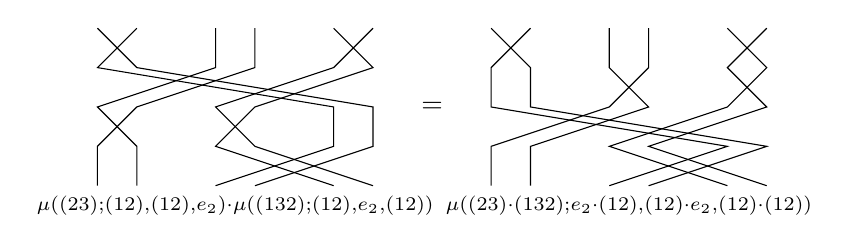
\begin{tikzpicture}[scale=0.5]
    \draw (1,0) -- (2,-1) -- (8,-2) -- (8,-3) -- (5,-4);
    \draw (2,0) -- (1,-1) -- (7,-2) -- (7,-3) -- (4,-4);
    \draw (4,0) -- (4,-1) -- (1,-2) -- (2,-3) -- (2,-4);
    \draw (5,0) -- (5,-1) -- (2,-2) -- (1,-3) -- (1,-4);
    \draw (7,0) -- (8,-1) -- (5,-2) -- (4,-3) -- (7,-4);
    \draw (8,0) -- (7,-1) -- (4,-2) -- (5,-3) -- (8,-4);
    %
    \node at (9.5,-2) {$=$};
    %
    \draw (11,0) -- (12,-1) -- (12,-2) -- (18,-3) -- (15,-4);
    \draw (12,0) -- (11,-1) -- (11,-2) -- (17,-3) -- (14,-4);
    \draw (14,0) -- (14,-1) -- (15,-2) -- (12,-3) -- (12,-4);
    \draw (15,0) -- (15,-1) -- (14,-2) -- (11,-3) -- (11,-4);
    \draw (17,0) -- (18,-1) -- (17,-2) -- (14,-3) -- (17,-4);
    \draw (18,0) -- (17,-1) -- (18,-2) -- (15,-3) -- (18,-4);
    %
    \node at (4.5,-4.5) {$\scriptstyle \mu\left((23);(12),(12), e_2\right) \cdot \mu\left((132); (12), e_2, (12)\right)$};
    \node at (14.5,-4.5) {$\scriptstyle \mu\left((23)\cdot (132); e_2 \cdot (12), (12) \cdot e_2, (12) \cdot (12)\right)$};
  \end{tikzpicture}
  \end{center}
\item Our definition of an action operad is the same as that appearing in Wahl's thesis \cite{wahl-thesis}, but without the condition that each $\pi_{n}$ is surjective. It is also the same as that appearing in work of Zhang \cite{zhang-grp}, although we prove later (see \cref{calclem}) that Zhang's condition of $e_{1} \in \Lambda(1)$ being the identity element follows from the rest of the axioms.
\item Yau \cite{yau_infinity_2021} collects together a large number of results on the topic of action operads while also investigating the setting of infinity group operads. 
\end{itemize}
\end{rem}

\begin{example}
\begin{enumerate}
\item The terminal operad $T$ in the category of sets has a unique action operad structure, $\mathbf{T}$. Since $T(n)$ is a singleton for each $n$, the group structure is unique, as is the map $\pi$. The single action operad axiom is then automatic as both sides of \cref{eqn:ao_axiom} are the unique element which happens to be the identity. This is the initial object in the category of action operads (see \cref{Defi:cat_aop} for the definition of morphisms in the category of action operads).
\item The symmetric operad $\Sigma$ has a canonical action operad structure. It is given by taking $\pi$ to be the identity map, and this action operad will be denoted $\mathbf{\Sigma}$. This is the terminal object in the category of action operads.
\item Two less trivial examples are given by the braid groups, $\Lambda = B$, and the ribbon braid groups, $\Lambda = RB$. (A ribbon braid is given, geometrically, as a braid with strands replaced by ribbons in which we allow full twists. The actual definition of the ribbon braid groups is as the fundamental group of a configuration space in which points have labels in the circle, $S^{1}$; see \cite{sal-wahl}.)  In each case, the homomorphism $\pi$ is given by taking underlying permutations, and the operad structure is given geometrically by using the procedure explained after \cref{broperad}. We refer the reader to \cite{fie-br} for more information about braided operads, and to \cite{sal-wahl, wahl-thesis} for information about the ribbon case.
\item The operad of $n$-fruit cactus groups defined by Henriques and Kamnitzer in \cite{hk-cobound} has an action operad structure that we will discuss in \cref{sec:examples}.
\end{enumerate}
\end{example}

\begin{Defi} For each $n \in \mathbb{N}$, the \emph{ribbon braid group} $RB_{n}$ is the group whose presentation is the same as that of the braid group $B_{n}$, except with the addition of $n$ new generators $t_1, \ldots, t_n$, known as the \emph{twists}. These twists all commute with one other, and also commute with all braids except in the following cases:
  \begin{align*}
    b_i \cdot t_i &= t_{i+1} \cdot b_i,\\
    b_i \cdot t_{i+1} &= t_i \cdot b_i.
  \end{align*}
The \emph{ribbon braid operad} $RB$ is then the operad made up of these groups in a way that extends the definition of the braid operad. In other words, the identity is still $e_1 \in RB_1$, and the operadic multiplication is built up in stages in exactly the same ways as in \cref{broperad}, but with some additional rules for dealing with twists. With regards to the tensor product, we have that for any twist $t_i \in RB_{n}$,
  \[
    t_i = e_{i-1} \otimes t \otimes e_{n-i}
  \]
where $t$ is the sole twist in $RB_1$, and for the `block twists' $t_{(m)}$ we again work recursively:
  \[
    t_{(0)} = e_n, \quad \quad \quad t_{(m+m')} = \left(t_{(m)} \otimes t_{(m')}\right) \cdot b_{(m', m)} \cdot b_{(m, m')}
  \]
\end{Defi}

Much as the symmetric groups can be represented by crossings of a collection of strings, and the braid groups by braidings of strings, the ribbon braid groups deal with the ways that one can braid together several flat ribbons, including the ability to twist a ribbon about its own axis by 360 degrees.
\begin{center} \begin{tabular}{ccc}
			\begin{tikzpicture}[baseline]
				\node(xl1) at (-0.7,1){};
				\node(xr1) at (-0.3,1){};
				\node(yl1) at (0.3,1){};
				\node(yr1) at (0.7,1){};
				\node(yl2) at (-0.7, -1){};
				\node(yr2) at (-0.3, -1){};
				\node(xl2) at (0.3, -1){};
				\node(xr2) at (0.7, -1){};
				\node(b) at (0,0)[circle,fill=white, minimum size=0.5cm]{};
       				\draw[rounded corners](xl1.north) to (-0.7,0.5) to (0.3,-0.5) to (xl2.south);
       				\draw[rounded corners](xr1.north) to (-0.3,0.5) to (0.7,-0.5) to (xr2.south);
				\begin{pgfonlayer}{bg}
				\draw[rounded corners](yl1.north) to (0.3, 0.5) to (-0.7, -0.5) to (yl2.south);
				\draw[rounded corners](yr1.north) to (0.7, 0.5) to (-0.3, -0.5) to (yr2.south);
    				\end{pgfonlayer}
				\draw(xl1.north) to (xr1.north);
				\draw(xl2.south) to (xr2.south);
				\draw(yl1.north) to (yr1.north);
				\draw(yl2.south) to (yr2.south);
			\end{tikzpicture} & \quad \quad \quad \quad \quad \quad \quad &
			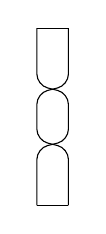
\begin{tikzpicture}[baseline]
				\node(xl1) at (-0.2,1){};
				\node(xr1) at (0.2,1){};	
				\node(xl2) at (-0.2, -1){};
				\node(xr2) at (0.2, -1){};
				\draw[rounded corners](xl1.north) to (-0.2,0.4) to (0.2, 0.3) to (0.2, -0.3) to (-0.2, -0.4) to (xl2.south);	
       				\draw[rounded corners](xr1.north) to (0.2,0.4) to (-0.2, 0.3) to (-0.2, -0.3) to (0.2, -0.4) to (xr2.south);
				\draw(xl1.north) to (xr1.north);
				\draw(xl2.south) to (xr2.south);	
			\end{tikzpicture} \\
			$b$ & & $t$ 
\end{tabular} \end{center}
This operad $RB$ is also clearly an action operad, since we can just define $\pi^{RB}_n \colon RB_{n} \rightarrow \Sigma_n$ to act like $\pi^B_n$ on any braids, at which point the fact that $\pi(t) \in S_1 = \{e_1\}$ will automatically take care of the twists.

\begin{example}
Every abelian group $A$ gives rise to action operad $A^{\bullet}$ as follows. The group $A^{\bullet}(n)$ is the direct sum of $n$ copies of $A$, $A^{n}$. The identity element is required to be $e \in A^{1}$, and the multiplication is defined by
  \[
    \mu((a_{1}, \ldots, a_{n}); \underline{b_1}, \ldots, \underline{b_n}) = (a_{1}+\underline{b_{1}}, a_{2} + \underline{b_{2}}, \ldots, a_{n} + \underline{b_{n}})
  \]
where $\underline{b_{i}}$ is the string $b_{i1}, \ldots, b_{ik_{i}}$, and $a_{i} + \underline{b_{i}}$ is
  \[
    a_{i} + b_{i1}, a_{i} + b_{i2}, \ldots, a_{i} + b_{ik_{i}}.
  \]
\end{example}


Action operads are themselves the objects of a category, $\mb{AOp}$. The morphisms of this category are defined below.
\begin{Defi}\label{mapaop}
A \textit{map of action operads} $f \colon  \Lambda \rightarrow \Lambda'$ consists of a map $f \colon \Lambda \rightarrow \Lambda'$ of the underlying operads such that
  \begin{enumerate}
    \item $\pi^{\Lambda'} \circ f = \pi^{\Lambda}$ (i.e., $f$ is a map of operads over $\Sigma$) and
    \item each $f_{n} \colon \Lambda(n) \rightarrow \Lambda'(n)$ is a group homomorphism.
  \end{enumerate}
\end{Defi}

\begin{Defi}\label{Defi:cat_aop}
The category $\mb{AOp}$ of action operads has objects which are action operads $\Lambda$ and
 morphisms $\Lambda \rightarrow \Lambda'$ as defined in \cref{mapaop}.
\end{Defi}

\subsection{Some algebra in action operads}
Here we begin to investigate the algebra of action operads, including a discussion of the group-like properties of action operads and their maps. For example, the notions of kernels, images, and short exact sequences are defined for action operads before comparing $\textbf{Grp}$-operads and crossed simplicial groups to action operads as well. We provide some useful technical lemmas and go on to give an algebraic characterisation of action operads given by equivariant analogues of block sums of permutations and diagonal maps.

 	% QQQ chapter: some algebra in action operads
 	% \begin{itemize}
 	% 	\item discusses group-like properties of action operads and their maps: kernels, short exact sequences, fitting Grp-operads into the picture
 	% 	\item some useful technical algebraic lemmas
 	% 	\item algebraic characterisation of action operads via $\beta$ and $\delta$ maps
 	% \end{itemize}

We begin with a simple proposition.

\begin{prop}
The map $\pi \colon \Lambda \rightarrow \Sigma$ is a map of action operads.
\end{prop}


\begin{prop}\label{Z}
There exists a functor $Z \colon  \mb{Op}(\mb{Grp}) \rightarrow \mb{AOp}$ from the category of operads in groups (using the cartesian monoidal structure) to the category of action operads. This functor is full, faithful, and its image is precisely the collection of action operads $\Lambda$ with $\pi_{n}(g) = e_{n}$ for all $n \in \mathbb{N}$, $g \in \Lambda(n)$.
\end{prop}
\begin{proof}
Given an operad in groups $P$, $Z(P)$ is the action operad with the same underlying operad and each $\pi_{n}$ the zero map. It is easy to verify that $\mu$ is a group homomorphism if and only if $\pi_{n}$ is zero for all $n$, and further that maps between such action operads are precisely the same thing as maps between the corresponding operads in the category of groups.
\end{proof}

We have the following corollary.
\begin{cor}\label{corZ}
For an action operad $\Lambda$, the sets
  \[
    \mathrm{Ker}\,\pi_n = \{g \in \Lambda(n)~\colon~\pi_{n}(g) = e_{n} \}
  \]
form an action operad for which the inclusion $\mathrm{Ker}\,\pi \hookrightarrow \Lambda$ is a map of action operads.
\end{cor}
\begin{proof}
For $\textrm{Ker}\,\pi \hookrightarrow \Lambda$ to be a map of action operads, we must define the map $\textrm{Ker}\,\pi \rightarrow \Sigma$ to be zero,  and we must check that the operadic multiplication of elements in the kernel is also in the kernel. This last fact is a trivial consequence of $\pi$ being an operad map.
\end{proof}
\begin{cor}\label{image}
For an action operad $\Lambda$, the sets
  \[
    \mathrm{Im}\,\pi_n = \{\pi_n(g)~\colon~g \in \Lambda(n)\}
  \]
form an action operad for which the inclusion $\mathrm{Im}\,\pi \hookrightarrow \Sigma$ is a map of action operads.
\end{cor}
\begin{proof}
The operad multiplication of elements in the image is also in the image, as is the unit element in $\mathrm{Im}\,\pi_1$, following again as a consequence of $\pi$ being an operad map. The map $\mathrm{Im}\,\pi \hookrightarrow \Sigma$ is an inclusion and so is immediately seen to be a map of action operads.
\end{proof}

\begin{prop}[Corollary 2.17,  \cite{zhang-grp}]\label{surjortriv}
The homomorphisms $\pi_n \colon \Lambda(n) \rightarrow \Sigma_n$ are either all surjective or all the zero map.
\end{prop}
\begin{proof}
We will prove each case separately. The two cases coincide for $n = 0$ and $n = 1$ as $\pi_0$ and $\pi_1$ are both the zero map and since $\Sigma_0$ and $\Sigma_1$ are the trivial group then these maps are also surjective.

Any homomorphism $G \rightarrow \Sigma_2$ must necessarily be surjective or the zero map. To begin we will show that if $\pi_2 \colon \Lambda(2) \rightarrow \Sigma_2$ is surjective then, by induction, the rest of the maps $\pi_n$ are also surjective. If $\pi_2$ is surjective then there exists an element $g_{1,1} \in \Lambda(2)$ such that $\pi_2(g_{1,1}) = \trans{1}{2}$. Now assume that for some $j \geq 2$ that $\pi_j$ is surjective. In particular, this means that for each transposition $\trans{a}{a+k} \in \Sigma_j$, where $1 \leq a \leq j-1$ and $a + k \leq j$, there exists $g_{a,k} \in \Lambda(j)$ such that $\pi_j(g_{a,k}) = \trans{a}{a+k}$. We will use these assumptions to show that each transposition in $\Sigma_{j+1}$ can be written as the image under $\pi_{j+1}$ of some element in $\Lambda(j+1)$, hence any permutation in $\Sigma_{j+1}$ can similarly be written.


Let $\trans{a}{a+k} \in \Sigma_j$, where $1 \leq a \leq j$ and $a + k \leq j+1$. If $a + k \leq j$, then $\trans{a}{a+k} = \trans{a}{a+k}(j + 1) \in \Sigma_{j+1}$. This transposition can be written as
  \begin{align*}
    \trans{a}{a+k} &= \mu^{\Sigma}(e_2 ; \trans{a}{a+k}, e_1) \\
              &= \mu^{\Sigma}(\pi_2(e_2); \pi_j(g_{a,k}), \pi_1(e_1)) \\
              &= \pi_{j+1}\left(\mu^{\Lambda}(e_2; g_{a,k},e_1)\right).
  \end{align*}
Similarly, if $a > 1$ then this transposition can be written as
  \begin{align*}
   \trans{a}{a+k} &= \mu^{\Sigma}(e_2 ; e_1, \trans{a-1}{a+k-1}) \\
              &= \mu^{\Sigma}(\pi_2(e_2); \pi_1(e_1), \pi_j(g_{a-1,k})) \\
              &= \pi_{j+1}\left(\mu^{\Lambda}(e_2; e_1, g_{a-1,k})\right).
  \end{align*}
Finally, if $a = j$ and $k = 1$, then $\trans{a}{a+k} = \trans{j}{j+1}$. This can be written as
  \begin{align*}
    (j \,\,\, j + 1) &= \mu^{\Sigma}(e_2 ; e_{j-1}, (1 \,\,\, 2)) \\
              &= \mu^{\Sigma}(\pi_2(e_2); \pi_{j-1}(e_{j-1}), \pi_2(g_{1,1})) \\
              &= \pi_{j+1}\left(\mu^{\Lambda}(e_2; e_{j-1}, g_{1,1})\right).
  \end{align*}
Hence $\pi_{j+1}$ is surjective and so all $\pi_n$ are surjective.

Now instead suppose that $\pi_2 \colon \Lambda(2) \rightarrow \Sigma_2$ is the zero map. Assume that $\pi_j \colon \Lambda(j) \rightarrow \Sigma_j$ is the zero map for some $j \geq 2$. Letting $\sigma \in \textrm{Im}\,\pi_{j+1}$, there exists $g \in \Lambda(j+1)$ such that $\pi_{j+1}(g) = \sigma$. We can then consider the elements $\mu^\Sigma(\sigma; \underline{e_1}, e_o, \underline{e_1})$ where $\underline{e_1}$ means a sequence of $e_1$'s and with $e_0$ in the $k$th position, with $1 \leq k \leq j + 1$. Now
  \begin{align*}
    \mu^\Sigma(\sigma; \underline{e_1}, e_o, \underline{e_1}) &= \mu^\Sigma(\pi_{j+1}(g); \underline{\pi_1(e_1)}, \pi_0(e_0), \underline{\pi_1(e_1)}) \\
    &= \pi_j(\mu^\Lambda(g; \underline{e_1}, e_0, \underline{e_1})) \\
    &= e_j.
  \end{align*}
We can think of this permutation as being $\sigma$ with the $k$th string removed - in \cref{rem:crossed} we comment on such `face' and `degeneracy' maps as used here, and see \cite{ber-simplicial} for a more careful treatment of this idea. Now each of these is the identity $e_j$, as shown above. This means that $\sigma$ must either have been the identity $e_{j+1}$ or a transposition of the form $\trans{a}{a+1}$, where $1 \leq a \leq j$.

If $\sigma$ is the identity $e_{j+1}$, then we are done since this would give $\textrm{Im}\,\pi_{j+1} = \{e_{j+1}\}$. Instead suppose that $\sigma = \trans{a}{a+1} \in \Sigma_{j + 1}$. Then if $1 < a \leq j$ we can use this to give
  \begin{align*}
    \trans{a-1}{a} &= \mu^\Sigma(\trans{a}{a+1}; e_0, \underline{e_1}) \\
    &= \mu^\Sigma(\pi_{j+1}(g);\pi_0(e_0), \underline{\pi_1(e_1)}) \\
    &= \pi_j(\mu^\Lambda(g; e_0, \underline{e_1})) \\
    &= e_j.
  \end{align*}
This gives a contradiction, hence $\sigma \neq \trans{a}{a+1}$ and must be the identity $e_{j+1}$.

Similarly, if $\sigma = \trans{1}{2} \in \Sigma_{j+1}$, then in $\Sigma_j$ we find that
  \begin{align*}
    \trans{1}{2} &= \mu^\Sigma(\trans{1}{2} ; \underline{e_1}, e_0) \\
    &= \mu^\Sigma(\pi_{j+1}(g); \underline{\pi_1(e_1)}, \pi_0(e_0)) \\
    &= \pi_j(\mu^\Lambda(g ; \underline{e_1}, e_0)) \\
    &= e_j.
  \end{align*}
Again, a contradiction, hence $\sigma = e_{j+1}$.
\end{proof}

\begin{cor}\label{extension}
Every action operad $\Lambda$ with nontrivial $\pi$ fits into a short exact sequence
  \[
    T \rightarrow \mathrm{Ker}\,\pi \hookrightarrow \Lambda \stackrel{\pi}{\longrightarrow} \Sigma \rightarrow T,
  \]
by which we mean this is a sequence of action operad maps which is an exact sequence of groups at each $n$.
\end{cor}

\begin{rem}
Thus we see that an action operad is either an operad in groups, or is an extension of $\Sigma$ by an operad in groups. This gives a simple proof that the operads of pure braids and pure ribbon braids are both operads in groups.
\end{rem}

\begin{rem}\label{rem:crossed}
The crossed simplicial groups of Fiedoriwicz and Loday \cite{FL91} are related to action operads in the following way. We can define a functor $C \colon \mathbf{AOp} \rightarrow \mathbf{CSGrp}$ from the category of action operads just described into the category of crossed simplicial groups. This functor takes an action operad $\Lambda$ and defines $C(\Lambda)(n) = \Lambda(n+1)$. The face and degeneracy maps of the underlying simplicial structure are defined using the operadic composition inherent to $\Lambda$ - the description of the maps via the operad structure can be viewed in a similar way to Construction 1.1 of \cite{Kra96}. This functor is, however, not faithful, nor is it conservative. (Recall that a functor $F \colon \mathcal{C} \rightarrow \mathcal{D}$ is conservative if when $Ff$ is an isomorphism in $\mathcal{D}$, then $f$ is an isomorphism in $\mathcal{C}$.)
\end{rem}
%Salvatore-Wahl:  Framed disks operads\ldots

We now study some of the structure on the groups $\Lambda(n)$ for small values of $n$. Recall that $e_{n}$ is the identity element in the group $\Lambda(n)$.

\begin{lem}\label{calclem}
Let $\Lambda$ be an action operad.
\begin{enumerate}
\item In $\Lambda(1)$, the unit element $e_{1}$ for the group structure is equal to the identity element for the operad structure, $\id$.
\item The equation
  \[
    \mu(e_{n}; e_{i_{1}}, \ldots, e_{i_{n}}) = e_{I}
  \]
holds for any natural numbers $n, i_{j}, I = \sum_{j=1}^n i_{j}$.
\item The group $\Lambda(1)$ is abelian.
\end{enumerate}
\end{lem}
\begin{proof}
For the first claim, let $g \in \Lambda(1)$. Then
  \begin{align*}
    g & = g \cdot e_{1} \\
    &= \mu(g; \id) \cdot \mu(\id; e_{1}) \\
    &= \mu(g \cdot \id; \id \cdot e_{1}) \\
    &= \mu(g \cdot \id; \id) \\
    &= g \cdot \id
  \end{align*}
using that $e_{1}$ is the unit element for the group structure, that $\id$ is a two-sided unit for operad multiplication, and the final axiom for an action operad together with the fact that the only element of the symmetric group $\Sigma_{1}$ is the identity permutation. Thus $g = g \cdot \id$, so $\id = e_{1}$.

For the second claim, write the operadic product as $\mu(e; \underline{e})$, and consider the square of this element. We find that
  \begin{align*}
    \mu(e; \underline{e}) \cdot \mu(e; \underline{e}) & = \mu(e \cdot e; \underline{e} \cdot \underline{e}) \\
    &= \mu(e; \underline{e}),
  \end{align*}
where the first equality follows from the last action operad axiom together with the fact that $e$ gets mapped to the identity permutation; here $\underline{e} \cdot \underline{e}$ is the sequence $e_{i_{1}} \cdot e_{i_{1}}, \ldots, e_{i_{n}} \cdot e_{i_{n}}$. Thus $\mu(e; \underline{e})$ is an idempotent element of the group $\Lambda(I)$, so must be the identity element $e_{I}$.

For the final claim, note that the specific operadic multiplication map $\mu \colon \Lambda(1) \times \Lambda(1) \rightarrow \Lambda(1)$ is a group homomorphism following from the action operad axioms, and $\id = e_{1}$ is a two-sided unit, so the Eckmann-Hilton argument shows that $\mu$ is actually group multiplication and that $\Lambda(1)$ is abelian.
\end{proof}

\begin{lem}\label{G0abel}
Let $\Lambda$ be an action operad. The group operation of $\Lambda(0)$ coincides with the operation 
  \[
    g, h \in \Lambda(0) \mapsto \mu(e_2; g, h)
  \]
arising from the operad structure. Furthermore, $\Lambda(0)$ is abelian.
\end{lem}
\begin{proof}
  Note first that
    \begin{align*}
      \mu(e_2; g, h) &= \mu(e_2 \cdot e_2; g \cdot e_0, e_0 \cdot h) \\
      &= \mu(e_2; g, e_0) \cdot \mu(e_2; e_0, h),
    \end{align*}
  so for the first claim that $\mu(e_2; g, h) = g \cdot h$ it will suffice to show that $\mu(e_2; g, e_0) = g$ and $\mu(e_2; e_0, h) = h$ for all $g, h \in \Lambda(0)$. We will use the fact that $\mu(e_0; ) = e_0$, which follows below from a similar argument found in the second part of \cref{calclem}.
    \begin{align*}
      \mu(e_0;)\mu(e_0;) &= \mu\left(e_0^2;\right) \\
      &= \mu(e_0;).
    \end{align*}
  Since $\mu(e_0;)$ is an idempotent element of $\Lambda(0)$, then it must be the identity $e_0$. Now we have this, the following sequence of calculations shows that $\mu(e_2; g, e_0) = g$, while a similar calculation would show that $\mu(e_2; e_0, h) = h$. Using \cref{calclem},
    \begin{align*}
      g &= \mu(e_1; g) \\
      &= \mu(\mu(e_2; e_0, e_1); g) \\
      &= \mu(e_2; \mu(e_0;), \mu(e_1; g)) \\
      &= \mu(e_2; e_0, g).
    \end{align*}
  It remains to show that $\Lambda(0)$ is abelian, which relies on the coincidence of the operad multiplication and the group operation in $\Lambda(0)$, in an Eckmann-Hilton style argument.
    \begin{align*}
      g \cdot h &= \mu(e_2; g, h) \\
      &= \mu(e_2 \cdot e_2; e_0 \cdot g, h \cdot e_0) \\
      &= \mu(e_2; e_0, h) \cdot \mu(e_2; g, e_0) \\
      &= h \cdot g.
    \end{align*}
\end{proof}

Note that the operad of symmetric groups $\Sigma$ has its action operad structure determined by two auxiliary operations, which we have previously used to describe particular types of operadic composition as described in \cref{conv1} and \cref{exSigma}. Rather than simply being convenient notation for common occurences of operadic composition, we will use these ideas to give a characterisation of action operads. First we recall these notions in more detail in the case of the symmetric operad $\Sigma$. The first operation is the block sum of permutations which we denote by
  \[
    \beta \colon \Sigma_{k_{1}} \times \cdots \times \Sigma_{k_{n}} \rightarrow \Sigma_{K},
  \]
where $K = \sum k_{i}$. The second is a kind of diagonal map which is defined for any natural number $n$ together with natural numbers $k_{1}, \ldots, k_{n}$. Then
  \[
    \delta = \delta_{n; k_{1}, \ldots, k_{n}} \colon \Sigma_{n} \rightarrow \Sigma_{K},
  \]
is defined on $\sigma \in \Sigma_{n}$ by permuting the elements $1, 2, \ldots, k_{1}$ together in a block according to the action of $\sigma \in \Sigma_{n}$ on $1$, then $k_{1}+1, \ldots, k_{1}+k_{2}$ together in a block according to the action of $\sigma$ on $2$, and so on. The first of these, $\beta$, is a group homomorphism, while $\delta$ is a sort of twisted homomorphism, and taken together they define operadic multiplication in $\Sigma$.

% \begin{Defi}\label{Defi:aop_bl}
% Let $\Lambda$ be an action operad. For $h_i \in \Lambda(k_i)$ and $g \in \Lambda(n)$, define
%   \begin{align*}
%     \beta(h_{1}, \ldots, h_{n}) &= \mu(e_n; h_{1}, \ldots, h_{n}), \\
%     \delta_{n; k_{1}, \ldots, k_{n}}(g) &= \mu(g; e_{k_1}, \ldots, e_{k_n}).
%   \end{align*}
% \end{Defi}


\begin{thm}\label{thm:charAOp}
An action operad $\Lambda$ determines, and is determined by, the following: 
\begin{itemize}
\item groups $\Lambda(n)$ together with group homomorphisms $\pi_{n} \colon \Lambda(n) \rightarrow \Sigma_{n}$,
\item a group homomorphism
  \[
    \Lambda(k_{1}) \times \cdots \times \Lambda(k_{n}) \stackrel{\beta}{\longrightarrow} \Lambda(k_{1} + \cdots + k_{n}),
  \]
for each $k_{1}, \ldots, k_{n}$ together with the degenerate case of $n=0$ which then is a group homomorphism $1 \rightarrow \Lambda(0)$, and
\item a function of sets
  \[
    \Lambda(n) \stackrel{\delta_{n; k_{1}, \ldots, k_{n}}}{\longrightarrow} \Lambda(k_{1} + \cdots + k_{n})
  \]
for each $n, k_{1}, \ldots, k_{n}$,
\end{itemize}
subject to the axioms below. In what we write below, we use the following notational conventions.
\begin{itemize}
\item The symbols $f,g,h$, with or without subscripts, always refer to an element of some group $\Lambda(n)$.
\item The symbols $j,k,m,n,p$ are all natural numbers, and $i$ is a natural number between 1 and $n$.
\end{itemize}
Axioms:
\begin{enumerate}
\item\label{eq1} The homomorphisms $\beta$ are natural with respect to the maps $\pi_{n}$, where $K = k_{1} + \cdots + k_{n}$.
  \[
    \xy
      (0,0)*+{\Lambda(k_{1}) \times \cdots \times \Lambda(k_{n}) } ="00";
      (0,-15)*+{\Sigma_{k_{1}} \times \cdots \times \Sigma_{k_{n}}  } ="01";
      (40,0)*+{\Lambda(K) } ="20";
      (40,-15)*+{\Sigma_{K} } ="21";
      {\ar^{\beta} "00" ; "20"};
      {\ar^{\pi} "20" ; "21"};
      {\ar_{\pi_1 \times \cdots \times \pi_n} "00" ; "01"};
      {\ar_{\beta} "01" ; "21"};
    \endxy
  \]

\item\label{eq2} The homomorphism $\beta \colon \Lambda(k) \rightarrow \Lambda(k)$ is the identity.
\item\label{eq3} The homomorphisms $\beta$ are associative in the sense that the equation
% \[
% \beta(h_{11}, \ldots, h_{1j_{1}}, h_{21}, \ldots, h_{2j_{2}}, \ldots, h_{nj_{n}}) = \beta\left( \beta(h_{11}, \ldots, h_{1j_{1}}), \ldots, \beta(h_{n1}, \ldots, h_{nj_{n}}) \right)
% \]
\[
  \beta(\underline{h_1},\ldots,\underline{h_n}) = \beta(\beta(\underline{h_1}),\ldots,\beta(\underline{h_n}))
\]
holds, where $\underline{h_i} = h_{i1},\ldots,h_{ij_i}$.
\item\label{eq4} The functions $\delta_{n; k_{1}, \ldots, k_{n}}$ are natural with respect to the maps $\pi_{n}$, where $K = k_1 + \cdots + k_n$.
  \[
    \xy
      (0,0)*+{\Lambda(n)} ="00";
      (40,0)*+{\Lambda(k_{1} + \cdots + k_{n}) } ="20";
      (0,-15)*+{\Sigma_{n}  } ="01";
      (40,-15)*+{\Sigma_{k_{1} + \cdots + k_{n}} } ="21";
      {\ar^{\delta} "00" ; "20"};
      {\ar^{\pi} "20" ; "21"};
      {\ar_{\pi} "00" ; "01"};
      {\ar_{\delta} "01" ; "21"};
    \endxy
  \]

\item\label{eq5} The functions $\delta_{n; 1, \ldots, 1}, \, \delta_{1;n} \colon \Lambda(n) \rightarrow \Lambda(n)$ are the identity.
\item\label{eq6} The equation $\delta_{n; k_{i}}(g) \delta_{n; j_{i}}(h) = \delta_{n; j_{i}}(gh)$ holds when
  \[
    k_{i} = j_{h^{-1}(i)}.
  \]
\item\label{eq7} The functions $\delta$ are associative in the sense that the equation
% \[
% \delta_{m_1 + \cdots + m_n; p_{11}, \ldots, p_{1m_{1}}, p_{21}, \ldots, p_{nm_{n}}}\left( \delta_{n; m_{1}, \ldots, m_{n}}(f) \right) = \delta_{n; P_{1}, \ldots, P_{n}}(f)
% \]
  \[
    \delta_{m_1 + \cdots + m_n; \underline{p_1},\ldots,\underline{p_n}}\left( \delta_{n; m_{1}, \ldots, m_{n}}(f) \right) = \delta_{n; P_{1}, \ldots, P_{n}}(f)
  \]
holds, where $P_{i} = p_{i1} + \cdots + p_{im_{i}}$ and $\underline{p_i} = p_{i1}, \ldots, p_{im_i}$.
\item\label{eq8} The equation
  \[
    \delta(g) \beta(h_{1}, \ldots, h_{n}) = \beta(h_{g^{-1}(1)}, \ldots,  h_{g^{-1}(n)}) \delta(g)
  \]
holds, where $h_{i} \in \Lambda(k_{i})$ and $\delta \colon \Lambda(n) \rightarrow \Lambda(k_{1} + \cdots + k_{n})$.
\item\label{eq9} The equation
  \[
    \beta(\delta_{1}(g_{1}), \ldots, \delta_{n}(g_{n})) = \delta_{c}(\beta(g_{1}, \ldots, g_{n}))
  \]
holds, where $\delta_{i}(g_{i})$ is shorthand for $\delta_{k_{i}; m_{i1}, \ldots, m_{ik_{i}}}(g_{i})$ and $\delta_{c}$ is shorthand for
  \[
    \delta_{k_{1}+\cdots + k_{n}; m_{11}, m_{12}, \ldots, m_{1k_{1}}, m_{21}, \ldots, m_{nk_{n}}}.
  \]
\end{enumerate}
\end{thm}

\begin{proof}
Let $\Lambda$ be an action operad, and define $\beta, \delta$ as in \cref{conv1}. Since $\pi \colon \Lambda \rightarrow \Sigma$ is an operad map, axioms \eqref{eq1} and \eqref{eq4} hold. Since $\Lambda$ is an operad of sets, axioms \eqref{eq2} and \eqref{eq5} follow from the operad unit axioms, and axioms \eqref{eq3}, \eqref{eq7}, and \eqref{eq9} follow from the operad associativity axiom. Axioms \eqref{eq6} and \eqref{eq8} are special cases of the additional action operad axiom, as is the fact that $\beta$ is a group homomorphism.

Conversely, given the data above, we need only define the operad multiplication, verify the operad unit and multiplication axioms,  and finally check the action operad axiom. Multiplication is given by
  \[
    \mu(g; h_{1}, \ldots, h_{n}) = \delta_{n; k_{1}, \ldots, k_{n}}(g) \beta(h_{1}, \ldots, h_{n})
  \]
where $h_{i} \in \Lambda(k_{i})$. The unit is $e \in \Lambda(1)$.

We now verify the operad unit axioms.
  \begin{align*}
    \mu(e; g) &= \delta(e)\beta(g) \\
    &= e \cdot g \\
    &= g \\
    \mu(h; e, \ldots, e) &= \delta(h)\beta(e, \ldots, e) \\
    &= h \cdot e \\
    &= h
  \end{align*}
These follow from axioms \eqref{eq2} and \eqref{eq5}, together with the fact that $\beta$ is a group homomorphism.

For the operad associativity axiom, let
\begin{itemize}
\item $f \in \Lambda(m),$
\item $g_{i} \in \Lambda(n_{i})$ for $i=1, \ldots, m$, and
\item $h_{ij} \in \Lambda(p_{i,j})$ for $i=1, \ldots, m$ and $j=1, \ldots, n_{i}$.
\end{itemize}
Further, let $P_{i} = p_{i1} + \cdots + p_{in_{i}}$ and $\underline{h_i}$ denote the list $h_{i1}, h_{i2}, \ldots, h_{in_{i}}$. We must then show that
  \[
    \mu\left( f; \mu\left(g_{1}; \underline{h_1}\right), \ldots, \mu\left(g_{m}; \underline{h_m}\right) \right) = \mu\left( \mu\left(f; g_{1}, \ldots, g_{m}\right); \underline{h_1}, \ldots, \underline{h_m} \right).
  \]
By definition, the left side of this equation is
  \[
    \delta_{m; P_{1}, \ldots, P_{m}}(f) \beta\left( \mu\left(g_{1}; \underline{h_1}\right), \ldots, \mu\left(g_{m}; \underline{h_m}\right) \right),
  \]
and
  \[
    \mu\left(g_{i}; \underline{h_i}\right) = \delta_{n_{i}; p_{i1}, \ldots, p_{in_{i}}}(g_{i})\beta\left(h_{i1}, \ldots, h_{in_{i}}\right).
  \]
Since $\beta$ is a group homomorphism, we can then rewrite the left side as
  \[
    \delta(f)\beta\left(\delta(g_{1}), \ldots, \delta(g_{m})\right)\beta\left(\beta\left(\underline{h_1}\right), \ldots, \beta\left(\underline{h_m}\right)\right)
  \]
where we have suppressed the subscripts on the $\delta$'s. By axiom \eqref{eq3},
  \[
    \beta\left(\beta\left(\underline{h_1}\right), \ldots, \beta\left(\underline{h_m}\right)\right) = \beta\left(\underline{h_1},\ldots,\underline{h_m}\right).
  \]
Further, axiom \eqref{eq9} above shows that
  \[
    \beta\left(\delta(g_{1}), \ldots, \delta\left(g_{m}\right)\right) = \delta\left(\beta\left(g_{1}, \ldots, g_{m}\right)\right).
  \]
Thus we have shown that the left side of the operad associativity axiom is equal to
  \[
    \delta(f)\delta\left(\beta(g_{1}, \ldots, g_{m})\right)\beta\left(\underline{h_1},\ldots,\underline{h_m}\right).
  \]
Now the right side is
  \[
    \mu\left( \mu (f; g_{1}, \ldots, g_{m}); \underline{h_1}, \ldots, \underline{h_m} \right)
  \]
which is by definition
  \[
    \delta\left(\mu (f; g_{1}, \ldots, g_{m})\right)\beta\left(\underline{h_1}, \ldots, \underline{h_m}\right).
  \]
Thus verifying the operad associativity axiom reduces to showing
\begin{eqn}\label{eqn:opass}
\delta(f)\delta\left(\beta(g_{1}, \ldots, g_{m})\right) = \delta\left(\mu (f; g_{1}, \ldots, g_{m})\right).
\end{eqn}By the definition of $\mu$,
  \[
    \delta(\mu (f; g_{1}, \ldots, g_{m})) = \delta\left(\delta(f)\beta(g_{1}, \ldots, g_{m}) \right)
  \]
which is itself equal to
\begin{eqn}\label{eqn:opass2}
\delta\left(\delta(f)\right) \delta\left(\beta(g_{1}, \ldots, g_{m})\right)
\end{eqn}by axiom \eqref{eq6} above. Now the $\delta(f)$ on the left side of \cref{eqn:opass} uses $\delta_{n; P_{1}, \ldots, P_{n}}$, while the $\delta(\delta(f))$ in \cref{eqn:opass2} is actually
  \[
    \delta_{m_1 + \cdots + m_{n}; q_{ij}}(\delta_{n; m_{1}, \ldots, m_{n}} (f))
  \]
where the $q_{ij}$ are defined, by axiom \eqref{eq6}, to be given by
  \[
    q_{ij} = p_{i,g_{i}^{-1}(j)}
  \]
using the compatibility of $\beta$ and $\pi$ in axiom \eqref{eq1}. By axiom \eqref{eq7}, this composite of $\delta$'s  is then $\delta_{n; Q_{1}, \ldots, Q_{n}}$ where $Q_{i} = q_{i1} + \cdots + q_{im_{i}}$. But by the definition of the $q_{ij}$, we immediately see that $Q_{i} = P_{i}$, so the $\delta(f)$ in \cref{eqn:opass} is equal to the $\delta(\delta(f))$ appearing in \cref{eqn:opass2}, concluding the proof of the operad associativity axiom.

Writing $\mu(g;\underline{h}) = \mu\left(g; h_{1}, \ldots, h_{n}\right)= $ and $\mu(g';\underline{h'}) = \mu\left(g'; h_{1}', \ldots, h_{n}'\right)$, the action operad axiom is now the calculation below, and uses axioms \eqref{eq4} and \eqref{eq8}.
\begin{small}
  \begin{align*}
    \mu(g;\underline{h})\mu(g';\underline{h'}) &= \delta\left(g\right) \beta\left(h_{1}, \ldots, h_{n}\right) \delta\left(g'\right) \beta\left(h_{1}', \ldots, h_{n}'\right) \\
    &= \delta\left(g\right) \delta\left(g'\right) \beta\left(h_{\pi\left(g'\right)(1)}, \ldots, h_{\pi\left(g'\right)(n)}\right)  \beta\left(h_{1}', \ldots, h_{n}'\right) \\
    &= \delta\left(gg'\right) \beta\left(h_{\pi\left(g'\right)(1)}h_{1}', \ldots, h_{\pi\left(g'\right)(n)}h_{n}'\right) \\
    &= \mu\left(gg'; h_{\pi\left(g'\right)(1)}h_{1}', \ldots, h_{\pi\left(g'\right)(n)}h_{n}'\right)
  \end{align*}
\end{small}
\end{proof}

% \begin{nota}\label{beta_to_oplus}
% Leaning more heavily into the interpretation that the operations denoted $\beta$ above are block sums, we also write $g_1 \oplus g_2 \oplus \cdots \oplus g_n$ for
% $\beta(g_1, g_2, \ldots, g_n)$.
% \end{nota}

\subsection{Presentations of action operads}\label{sec:presofacops}
A useful method for constructing new examples of some given algebraic structure is through the use of presentations. A presentation consists of generating data together with relations between generators using the operations of the algebra involved. In categorical terms, the generators and relations are both given as free gadgets on some underlying data, and the presentation itself is a coequalizer. This section will establish the categorical structure necessary to give presentations for action operads, and then explain how such a presentation is reflected in the associated club and $2$-monad. The most direct route to the desired results uses the theory of locally finitely presentable categories. We recall the main definitions briefly, but refer the reader to \cite{ar} for additional details.

\begin{Defi}\label{def:filtered}
  A \textit{filtered category} is a nonempty category $C$ such that
    \begin{itemize}
      \item if $a,b$ are objects of $C$, then there exists another object $c \in C$ and morphisms $a \rightarrow c, b \rightarrow c$; and
      \item if $f,g \colon a \rightarrow b$ are parallel morphisms in $C$, then there exists a morphism $h \colon b \rightarrow c$ such that $hf = hg$.
    \end{itemize}
\end{Defi}

\begin{Defi}
  A \emph{filtered colimit} is a colimit over a filtered category.
\end{Defi}

\begin{Defi}
  Let $C$ be a category with all filtered colimits. An object $x \in C$ is \textit{finitely presentable} if the representable functor $C(x, -) \colon C \rightarrow \mb{Sets}$ preserves filtered colimits.
\end{Defi}

\begin{Defi}
  A \textit{locally finitely presentable category} is a category $C$ such that
  \begin{itemize}
    \item $C$ is cocomplete and
    \item there exists a small subcategory $C_{fp} \subseteq C$ of finitely presentable objects such that any object $x \in C$ is the filtered colimit of some diagram in $C_{fp}$.
  \end{itemize}
\end{Defi}

The definition of a locally finitely presentable category has many equivalent variants, but we find this one most practicable to work with in this setting.

\begin{thm}
The category $\mb{AOp}$ is locally finitely presentable.
\end{thm}
\begin{proof}
First note that we can define a category $\mb{Op}^{g}$, whose objects are operads $P$ in which each $P(n)$ also carries a group structure. This is an equational theory using equations with only finitely many elements, so $\mb{Op}^{g}$ is locally finitely presentable \cite[Corollary 3.7]{ar}. A slice category of a locally finitely presentable category is itself locally finite presentable \cite[Proposition 1.57]{ar} and since the symmetric operad is an object of $\mb{Op}^{g}$, the slice category $\mb{Op}^{g}/\Sigma$ is locally finitely presentable.

There is an obvious inclusion functor $\mb{AOp} \hookrightarrow \mb{Op}^{g}/\Sigma$. Now $\mb{AOp}$ is a full subcategory of $\mb{Op}^{g}/\Sigma$ which is closed under products, subobjects. Since any object of $\mb{Op}^{g}/\Sigma$ isomorphic to an action operad is in fact an action operad, the inclusion   $\mb{AOp} \hookrightarrow \mb{Op}^{g}/\Sigma$ is actually the inclusion of a reflective subcategory. One can easily check that $\mb{AOp}$ is in fact closed under all limits and filtered colimits in $\mb{Op}^{g}/\Sigma$, so by the Reflection Theorem (2.48 in \cite{ar}), $\mb{AOp}$ is locally finitely presentable.
\end{proof}

\begin{Defi}
  Let $\SS$ be the set which is the disjoint union of the underlying sets of all the symmetric groups. Then $\mb{Sets}/\SS$ is the slice category over $\SS$ with objects $(X,f)$ where $X$ is a set and $f \colon X \rightarrow \SS$ and morphisms $(X_{1}, f_{1}) \rightarrow (X_{2}, f_{2})$ are those functions $g \colon X_{1} \rightarrow X_{2}$ such that $f_{1} = f_{2}g$. We call an object $(X,f)$ a \textit{collection over $\SS$}.
\end{Defi}

\begin{rem}
In standard presentations of the theory of operads (see, for example, \cite{mss-op}), a nonsymmetric operad will have an underlying collection (or $\mathbb{N}$-indexed collection of sets) while a symmetric operad will have an underlying symmetric collection (or $\mathbb{N}$-indexed collection of sets in which the $n$th set has an action of $\Sigma_{n}$). Our collections over $\SS$ more closely resemble the former as there is no group action present.
\end{rem}

\begin{example}
One can easily form new action operads from old ones by taking limits. To take a limit of a diagram in $\mb{AOp}$, one forgets down to the category of operads over $\Sigma$ and takes the limit there. Concretely, products in $\mb{AOp}$ are computed as products in $\mb{Op}/\Sigma$ which themselves are (possibly wide) pullbacks in the category of operads. This pullback will then be computed levelwise, showing that at each dimension there is a group structure with a group homomorphism to the appropriate $\Sigma_{n}$ and that the final action operad axiom holds since it does in each component. The equalizer of a pair of maps will then just be the levelwise equalizer. This shows that the pointwise product of an action operad $P$ with an action operad of the form $Z(Q)$ (as in \cref{Z}) is again an action operad, but the pointwise product of two arbitrary action operads might not be.
\end{example}
\begin{thm}\label{underlyingSS}
There exists a forgetful functor $U \colon \mb{AOp} \rightarrow \mb{Sets}/\SS$ which preserves all limits and filtered colimits.
\end{thm}

\begin{proof}
For a given action operad $\Lambda$, we put $U(\Lambda) = \left(\coprod_{\mathbb{N}} \Lambda(n), \coprod_{\mathbb{N}} \pi_n \right)$ and this easily extends to a mapping on morphisms using the universal property of the coproduct. The preservation of filtered colimits follows from the fact that these are computed pointwise, together with the fact that every map between action operads preserves underlying permutations.
As equalizers are computed levelwise, and the product $\Lambda \times \Lambda'$ has underlying operad the pullback $\Lambda \times_{\Sigma} \Lambda'$; this pullback is itself computed levelwise. Together, these imply that $U$ also preserves all limits.
\end{proof}

\begin{cor}
$U$ has a left adjoint $F \colon \mb{Sets}/\SS \rightarrow \mb{AOp}$, the free action operad functor.
\end{cor}
\begin{proof}
The category $\mb{Sets}/\SS$ is locally finitely presentable as it is equivalent to the functor category $[\SS, \mb{Sets}]$ (here $\SS$ is treated as a discrete category) and any presheaf category is locally finitely presentable. The functor $U$ preserves limits and filtered colimits between locally finitely presentable categories, so has a left adjoint (see Theorem 1.66 in \cite{ar}).
\end{proof}

\begin{Defi}
  A \textit{presentation} for an action operad $\Lambda$ consists of
  \begin{itemize}
    \item a pair of collections over $\SS$ denoted $\mathbf{g}, \mathbf{r}$,
    \item a pair of maps $s_{1}, s_{2} \colon F\mathbf{r} \rightarrow F\mathbf{g}$ between the associated free action operads, and
    \item a map $p \colon F\mathbf{g} \rightarrow \Lambda$ of action operads exhibiting $\Lambda$ as the coequalizer of $s_{1},s_{2}$.
  \end{itemize}
\end{Defi}







